\documentclass{kupaper}
\usepackage{jtygm}%%%%%%%%%%%%%%%%%Font Warning対策%%%%%
\usepackage[dvipdfmx]{graphicx}
\usepackage{bmpsize}
\usepackage{here}
\usepackage{comment}
\usepackage{amsmath}
\usepackage{booktabs}
\usepackage[dvipdfmx,colorlinks=false]{hyperref}
\usepackage{titlesec}
\usepackage{wrapfig}
\usepackage{enumerate}

\begin{document}

%%% includeはできるだけつかわないでください!! 

\Title{論文執筆の手引き}
\Author{熊本 太郎}
\Date{7}{2}{13} %2024 卒論用
\Date{7}{2}{7}  %2024 修論用

\title{How to write a master's thesis}
\author{Taro Kumamoto}
\endate{February}{13}{2025} %2024 卒論用
\endate{February}{7}{2025}  %2024 修論用

%学部の人は次のコメント行の%を外してください.
%\senior 
%この\seniorは\Abstractの前であればどこに書いてもかまいません.

\Maketitle


\begin{Abstract}
	ここでは,研究全体に関する概要を書きます.しっかりと結論も書きましょう.
\end{Abstract}

\begin{abstract}
	%学部の人は書く必要ありません.
	%Write abstract of your entire research. Do not forget to write the  conclusion. 
\end{abstract}

%\setcounter{chapter}{20}
% 目次  (LaTeX の処理を少くする目的で,最後に書いています)
\pagenumbering{roman}
\setcounter{page}{1}
\tableofcontents

\begin{comment} %必要に応じて利用してください.
\clearpage
\listoffigures
\clearpage
\listoftables
\end{comment}

\chapter{はじめに}
\pagenumbering{arabic} % 絶対必要です.最初の章にのみ記述します.

卒業論文・修士論文は,みなさんのこれまでの研究の成果をまとめて報告し,みなさんがそれぞれの学位に値するかを審査するための重要な論文です.そのためには,これまでの研究成果の内容をよく吟味し,「人に自分の考えを伝える」重要性と難しさに注意し,分かりやすい表現を考え,書いた文章をよく推敲し,さらに,論文として定められた形式をとる必要があります.
\chapter{メディアおよび必要部数}
\begin{itemize}
	\item 卒業論文:冊子体1部および電子版 (PDFファイル) 
	\item 修士論文:冊子体3部\footnote{論文審査委員が4名以上の場合は,その人数分の部数を準備すること.}および電子版 (PDFファイル) 
\end{itemize}

\chapter{提出および投稿の締切日時}
\begin{itemize}
	\item 卒業論文:2025年 2月 6日 (木) 17時 (発表会は 2月13日(木))
	\item 修士論文:2025年 1月30日 (金)17時 (試問会は 2月 6日(木)~ 2月 7日(金))
\end{itemize}
ただし電子版は修正箇所がある場合,発表会・試問会の前日17時まで再投稿が可能です.

\chapter{提出先および投稿先}
提出可能時期については,各年度の執筆要領を参照してください.
\begin{itemize}
	\item 冊子体:指導教員,副指導教員
	\item 電子版:\url{http://www.st.cs.kumamoto-u.ac.jp/ronbun/} 
\end{itemize}

\chapter{冊子体の体裁}



冊子体は電子版と全く同じ内容の文書を印刷し,製本したものとします.製本には市販の簡易ファイル等を使ってください.製本完成時の全体の体裁を図1に示します.指導教員の指導に従い,表表紙および背表紙には所定の事項を記載し綴じてください.所定の事項は,黒色のペンを用いて手書きするか,プリンタで印字したものを貼付けてください.製本の際には,論文の左側約 13 mmの位置に孔を二つ開けて綴じてください.

\begin{figure}[htbp]
	\centering
	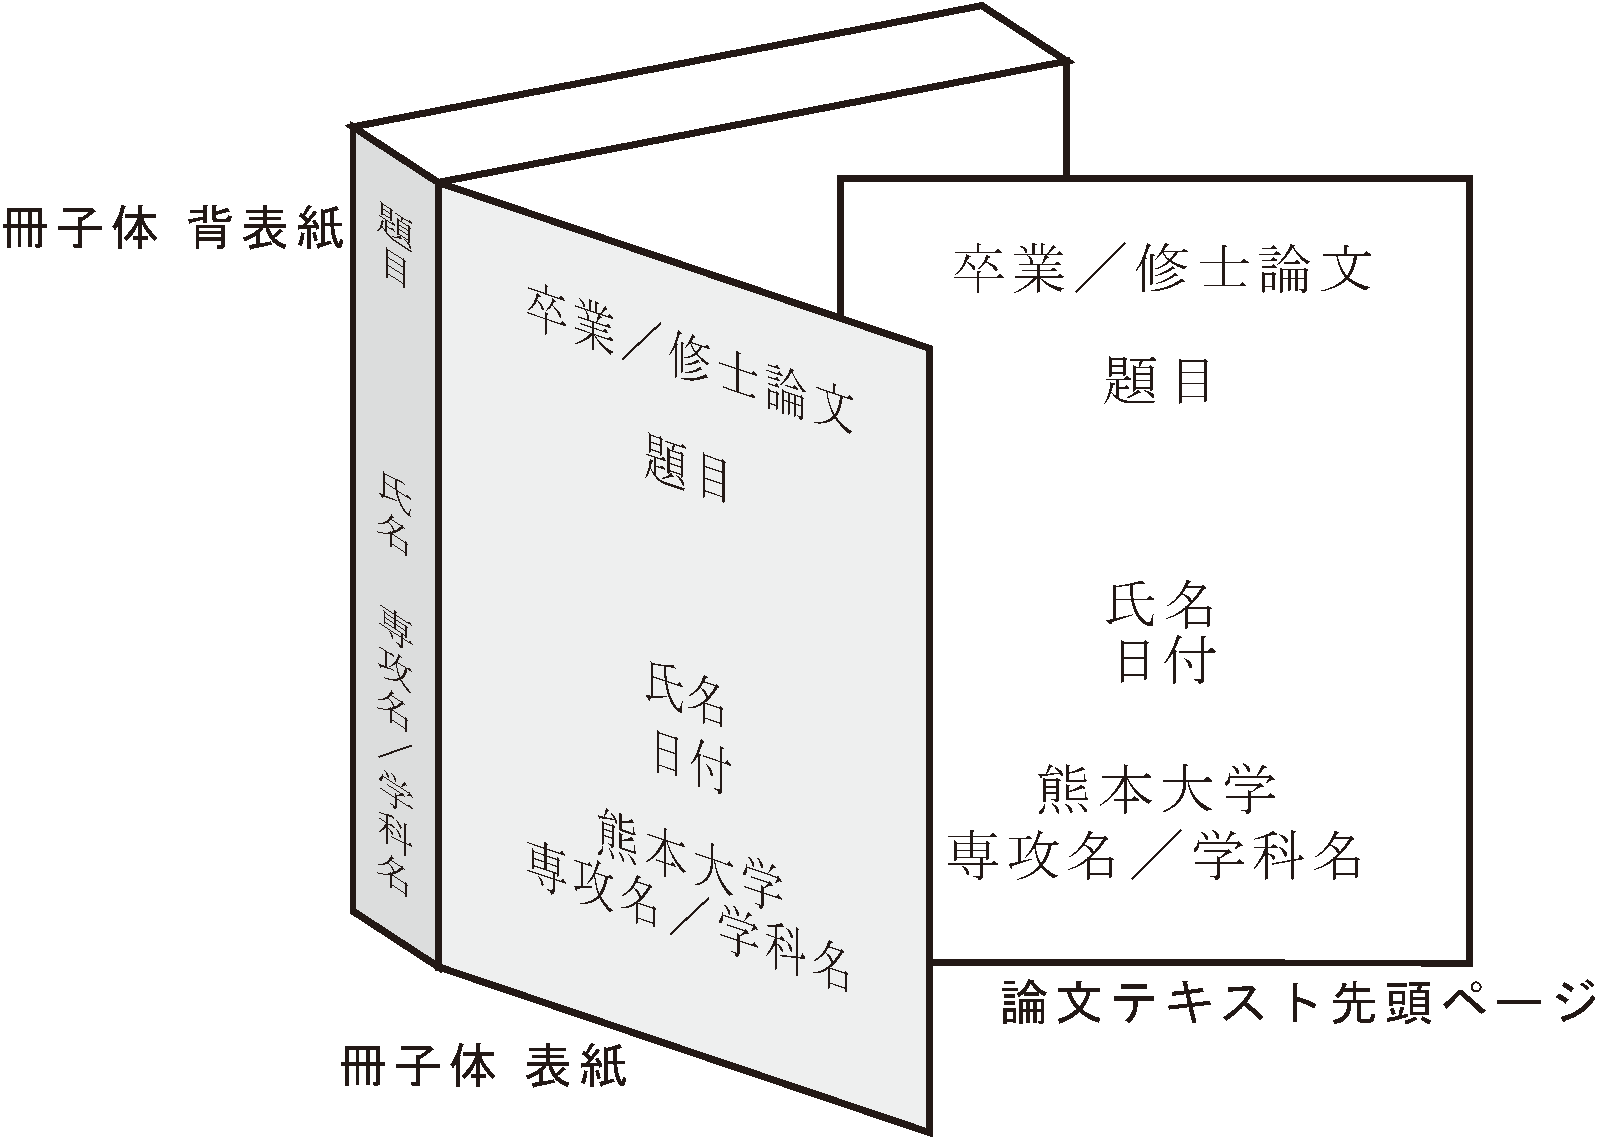
\includegraphics[width=1.0\linewidth,keepaspectratio]{book.pdf}
	\caption{冊子体および論文テキストの先頭ページ}
	\label{overview}
\end{figure}

%\vspace*{-3em}
なお,論文テキストの先頭ページには題目・氏名・日付 (試問会または発表会の最終日) ・大学名・学科 (専攻) 名を記載してください.これらの印字位置は図\ref{overview}に従って調整してください.


\chapter{論文の構成} \label{論文の構成}
論文は,以下の\ref{a}~\ref{f}の順序で構成してください.



\begin{enumerate}[a.]
	\item 論文テキスト先頭ページ:図\ref{overview}のように記載してください.\label{a}
	\item 概要\label{b}
	      卒業論文の場合:1ページ以内の論文概要
	      修士論文の場合:後述の7.に従って作成した論文概要.和文と英文の両方が必要です.
	\item 目次\label{c}
	\item 本文\label{d}
	\item 謝辞\label{e}
	\item 参考文献\label{f}
\end{enumerate}

\chapter{論文の記述要領}
\begin{enumerate}[a.]
	\item 文書作成ソフトウェア等で作成してください.なお,電子版はPDF形式で投稿してください.
	\item 用紙のサイズはA4版とし,縦長・横書きを基本とします.
	\item 用紙の上下左右に 30 mmずつ余白を取り,その内部のみに記載してください.
	\item \ref{論文の構成} の\ref{a},\ref{b}にはページ番号を付けないでください.\ref{c}にはローマ数字の小文字 (i,ii,...) を使ってページ番号を付けてください.\ref{d},\ref{e},\ref{f}は,アラビア数字 (1,2,...) を使って通しでページ番号を付けてください.
	\item ページ番号は本文の右上部に記載してください.\ref{c}で規定した記載枠からはみ出さないようにしてください.
	\item 文章は和文 (常用漢字・現代ひらがな) あるいは英文のいずれか一方で統一して書いてください (修士論文の論文概要を除きます) .
	\item 術語は原則として各研究室に関連の深い学会の論文執筆基準に従ってください.また人名,書名,学会名等の固有名詞は,原語のまま用いてください.
	\item 本文中で文献を引用する際には,引用箇所に,数字を[ ] (左右の半大カッコ) で括って記載するか,上付き文字で数字をカッコ内に入れて記載し,参考文献の欄にその数字と文献の著者,書名 (表題) ,出典 (論文誌名等,巻号,ページ) ,発表年 (西暦) を記載してください.参考文献の記載の様式は,電気学会や電子情報通信学会等,各研究室に関連の深い学会の論文誌の執筆規定に準じてください.なお,関連の深い学会の論文誌の執筆規定で,引用箇所を数字でなく, (著者,発表年) などで表すこととされている場合は,その書き方でも構いません ((例3)を参照) .
	      	      
	      \begin{enumerate}[(例1)]
	      	\item 
	      	      分かりやすい簡潔な表現[5]を心掛けることは,論文執筆において重要なことである.\\
	      	      {[5]} 木下是雄,「理科系の作文技術」,中央公論社 中公新書624,pp.118-152,1981.
	      	\item 
	      	      分かりやすい簡潔な表現(5)を心掛けることは,論文執筆において重要なことである.\\
	      	      (5) 木下是雄,「理科系の作文技術」,中央公論社 中公新書624,pp.118-152,1981.
	      	\item \label{例3}
	      	      分かりやすい簡潔な表現 (木下,1981) を心掛けることは,…
	      	      (木下,1981)  \\
	      	      木下是雄,「理科系の作文技術」,中央公論社 中公新書624,pp.118-152 1981.\\
	      	      ※(例3)の場合,参考文献リストは,著者のABC順に,同一著者は執筆年順に並べる.
	      \end{enumerate}
	      	      
	\item 図表等の番号と表題は,図や写真の場合には図や写真の下に,表の場合には表の上に記載します.
	\item その他のことについては,論文の書き方を説明した \cite{木下是雄2001理科系の作文技術,学術論文の書き方・発表の仕方,howtocite} のような文献を参考にしてください.\\

\end{enumerate}

\chapter{修士論文の論文概要}
修士論文については和文と英文の論文概要を次の要領で作成してください.英文で本文を記述した場合も,論文概要は和文,英文の両方で作成することが望ましいです.詳細は指導教員の指示に従ってください.

\begin{enumerate}[1.]
	\item 論文概要 (和文) の形式
	      \begin{enumerate}[(1)]
	      	\item 表紙として,図2に示す修士論文テキストの先頭ページと同じ体裁で作った表紙を付けます.ただし,題目と氏名の間の行に,「論文概要」と書き添えてください.
	      	\item 研究の目的,論文全体のあらまし,各章の内容 (簡単に) ,結論 (やや詳しく) ,得られた成果の意義を,この順序で数ページ程度にまとめてください.
	      \end{enumerate}
	\item 論文概要 (英文) の形式
	      \begin{enumerate}[(1)]
	      	\item 表紙として,図2に示す修士論文テキストの先頭ページと同じ体裁で作った表紙を,英文で記載して付けます.ただし,題目と氏名の間の行に,Synopsisと書き添えてください.
	      	      更に,大学名・専攻名は,Department of Computer Science and Electrical Engineering, Graduate School of Science and Technology, Kumamoto University と記載してください.
	      	\item 研究の目的,論文全体のあらまし,結論を,若干ページ程度にまとめてください.
	      \end{enumerate}
	\item 和文,英文の英文概要とも目次は付けないでください.また,原則として,図,表,式を用いないでください.
\end{enumerate}


%謝辞
\begin{thanks}
	本論文を執筆するにあたり,感謝すべき人物,環境などがありましたら記述してください.
\end{thanks}

% 参考文献
\bibliography{ref}
\bibliographystyle{junsrt}
%\nocite{*}

\end{document}